\documentclass[12pt]{article}
 
\newenvironment{sol}[1][Solution]{\begin{trivlist}\item[\hskip\labelsep {\bfseries #1:}]}{\end{trivlist}}
\usepackage{minted}
%\usemintedstyle{perldoc}
\usemintedstyle{vs}
\usepackage{graphicx}
\graphicspath{./}

\usepackage[margin=1in]{geometry} 
\usepackage{amsmath,amsthm,amssymb}
\usepackage{times,url}
\usepackage{tikz}
\usepackage{color}
\usepackage{enumerate}
\begin{document}
\renewcommand{\qedsymbol}{\filledbox}
\begin{center}
    \textbf{CS 5/7350 - Test\#3} \\
    \textbf{November 30, 2022}
%replace X with the appropriate number
\end{center}
\begin{flushright}
Name: \underline{Bingying Liang }\\
ID:  \underline{\ \ \ \ \ 48999397 \ \ \ \ \ }
\end{flushright}

\begin{enumerate}
    \item \ [8 pts] Answer the following questions:
    \begin{enumerate}
        \item A program requires 1000s to process an input size of C = 7 and S =
700. If the running time is $\Theta (C * S) $about how long would it take to process an input size of C=14 and S=700?
    \begin{sol}
        2000s
    \end{sol}
    \item A program requires 1000s to process an input size of C = 7 and S = 700. If the running time is $\Theta (C * S) $ about how long would it take to process an input size of C=7 and S=1400?
    \begin{sol}
        2000s
    \end{sol}
    \item A program requires 1000s to process an input size of C = 7 and S = 700. If the running time is $ \Theta(C + S) $ about how long would it take to process an input size of C=7 and S=1400?
    \begin{sol}
        $\frac{1407}{707}\times 1000  \approx 1990.99s$
    \end{sol}
    \item A program requires 1000s to process an input size of C = 7 and S = 700. If the running time is $\Theta (C * S^2)$ about how long would it take to process an input size of C=7 and S=1400?
    \begin{sol}
        4000s
    \end{sol}
    \item A program requires 1000s to process an input size of C = 7 and S = 700. If the running time is $\Theta (2^{CS})$ about how long would it take to process an input size of C=7 and S=1400?
    \begin{sol}
        $2^{4900} \times 1000s$
    \end{sol}
    \end{enumerate}
    \textcolor{red}{\item \ [6 pts] Use the DGT algorithm discussed in class to determine how to represent the value 689 using the number system $ \beta=5, D = \{ -1, 0, 2, 3 ,6 \}$. Show your work.}
    \begin{sol}
    $-1 \bmod 5 = 4, 6 \bmod 5 = 1 $
    \begin{align*}
        & 689 \bmod 5 = 4 \rightarrow -1\\
        & 689 - (-1) = 690 \\
        & 690 \div 5 = 138 \\
        & ----------------- \\
        & 138 \bmod 5 = 3 \\
        & 138 - 3 = 135 \\
        & 135 \div 5 = 27 \\
        & ----------------- \\
        & 27 \bmod 5 = 2 \\
        & 27 - 2 = 25 \\
        & 25 \div 5 = 5 \\ 
        & ----------------- \\
        & 5 \bmod 5 = 0\\
        & 5 - 0 = 5\\
        & 5 \div 5 = 1\\
        & -------------------\\
        & 1 \bmod 5 = 1 \rightarrow 6\\
        & 1 - 6 = -5\\
        & -5 \div 5 = -1\\
        & -------------------\\
        & -1 \bmod 5 = -1 \\
        & -1 - (-1) = 0 \\
    \end{align*}
    \begin{align*}
        \therefore \bar{1}6023\bar{1}
    \end{align*}

    \end{sol}

    \item \ [8 pts] Give the asymptotic running time supported by the following tables:
    \begin{center}
    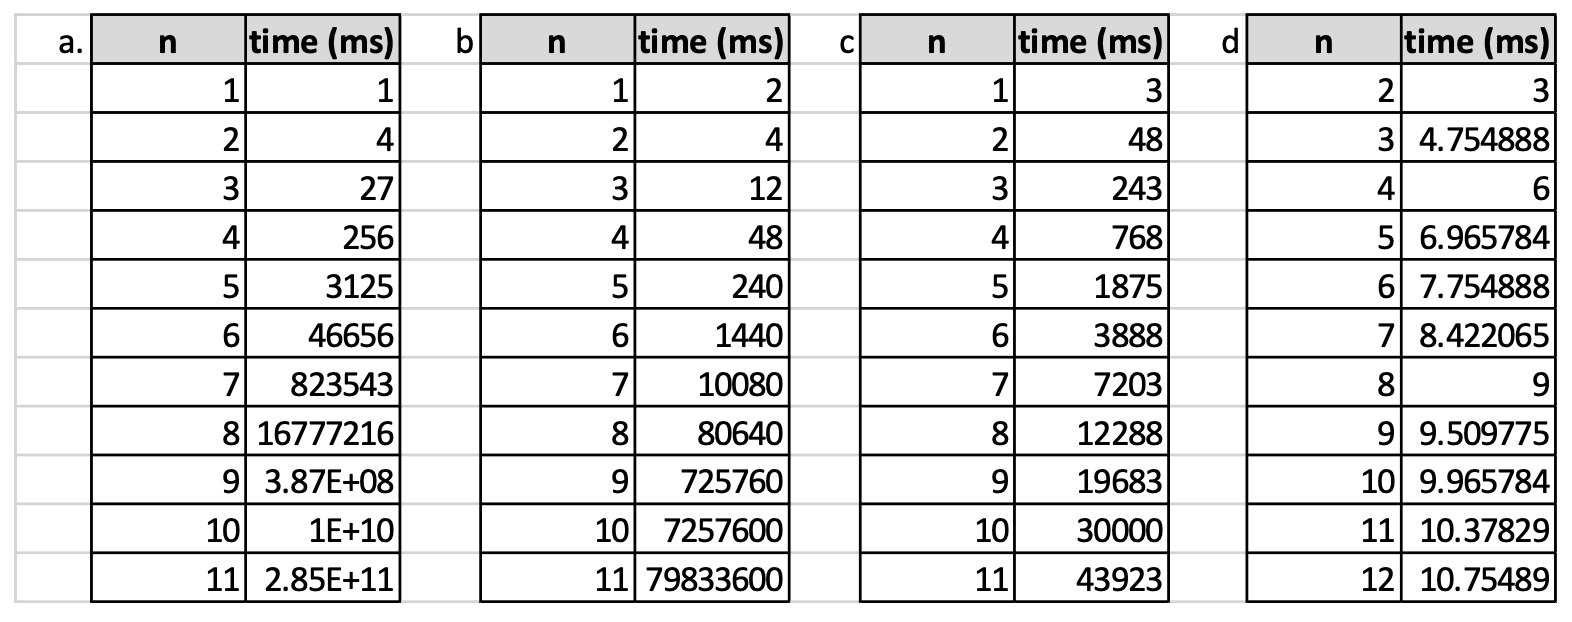
\includegraphics[width=0.9\textwidth]{p1.png}
    \end{center} 
    \begin{enumerate}
        \item $\Theta(n^n)$
        \item $n!$
        \item $n^4$
        \item $\log_2(n)$
    \end{enumerate}
    \textcolor{red}{\item \ [10 pts] Consider the following NP completeness questions. Answer them with the best answer of ``some” ``all” ``none” or ``unknown”}
    \begin{enumerate}
        \item Which Problems in P are also in NP? (“some” “all” “none” or “unknown”)
        \begin{sol}
            all
        \end{sol}
        \item Which Problems in NP are also in P? (“some” “all” “none” or “unknown”)
        \begin{sol}
            unknown
        \end{sol}
\item \textcolor{red}{ Which Problems in NP-Hard are also in NP? ( “some” “all” “none” “unknown” )
        \begin{sol}
            some
        \end{sol}} % unknown
        \item Which Problems in NP-Hard are also in NP-Complete ( “some” “all” “none” or “unknown”)
        \begin{sol}
            some
        \end{sol}
        \item The set of problems matching question (c) is exactly the same as the set of problems matching question (d) (true or false)
        \begin{sol}
            true
        \end{sol}
        \item If someone can solve an NP-Hard problem in Polynomial Time, then all NP problems can be solved in polynomial time. (true or false)
        \begin{sol}
        true
        \end{sol}
        \item If someone can solve an NP-Complete problem in Polynomial Time, then all NP and all NP-Complete problems can be solved in polynomial time. (true or false)
        \begin{sol}
            true
        \end{sol}
        \item At least 1 NP problem can be solved in polynomial time? (True or False)
        \begin{sol}
            true
        \end{sol}
        \item Which NP-Hard Problems are also NP-Complete? ( “some” “all” “none” or “unknown”)
        \begin{sol}
        some
        \end{sol}
        \item To show a problem is NP-Complete, you must show it is NP and that a solver for that problem can also solve some other NP-Complete problem with polynomial extra time. (True or False)
        \begin{sol}
            true
        \end{sol}
    \end{enumerate}
        \begin{center}
    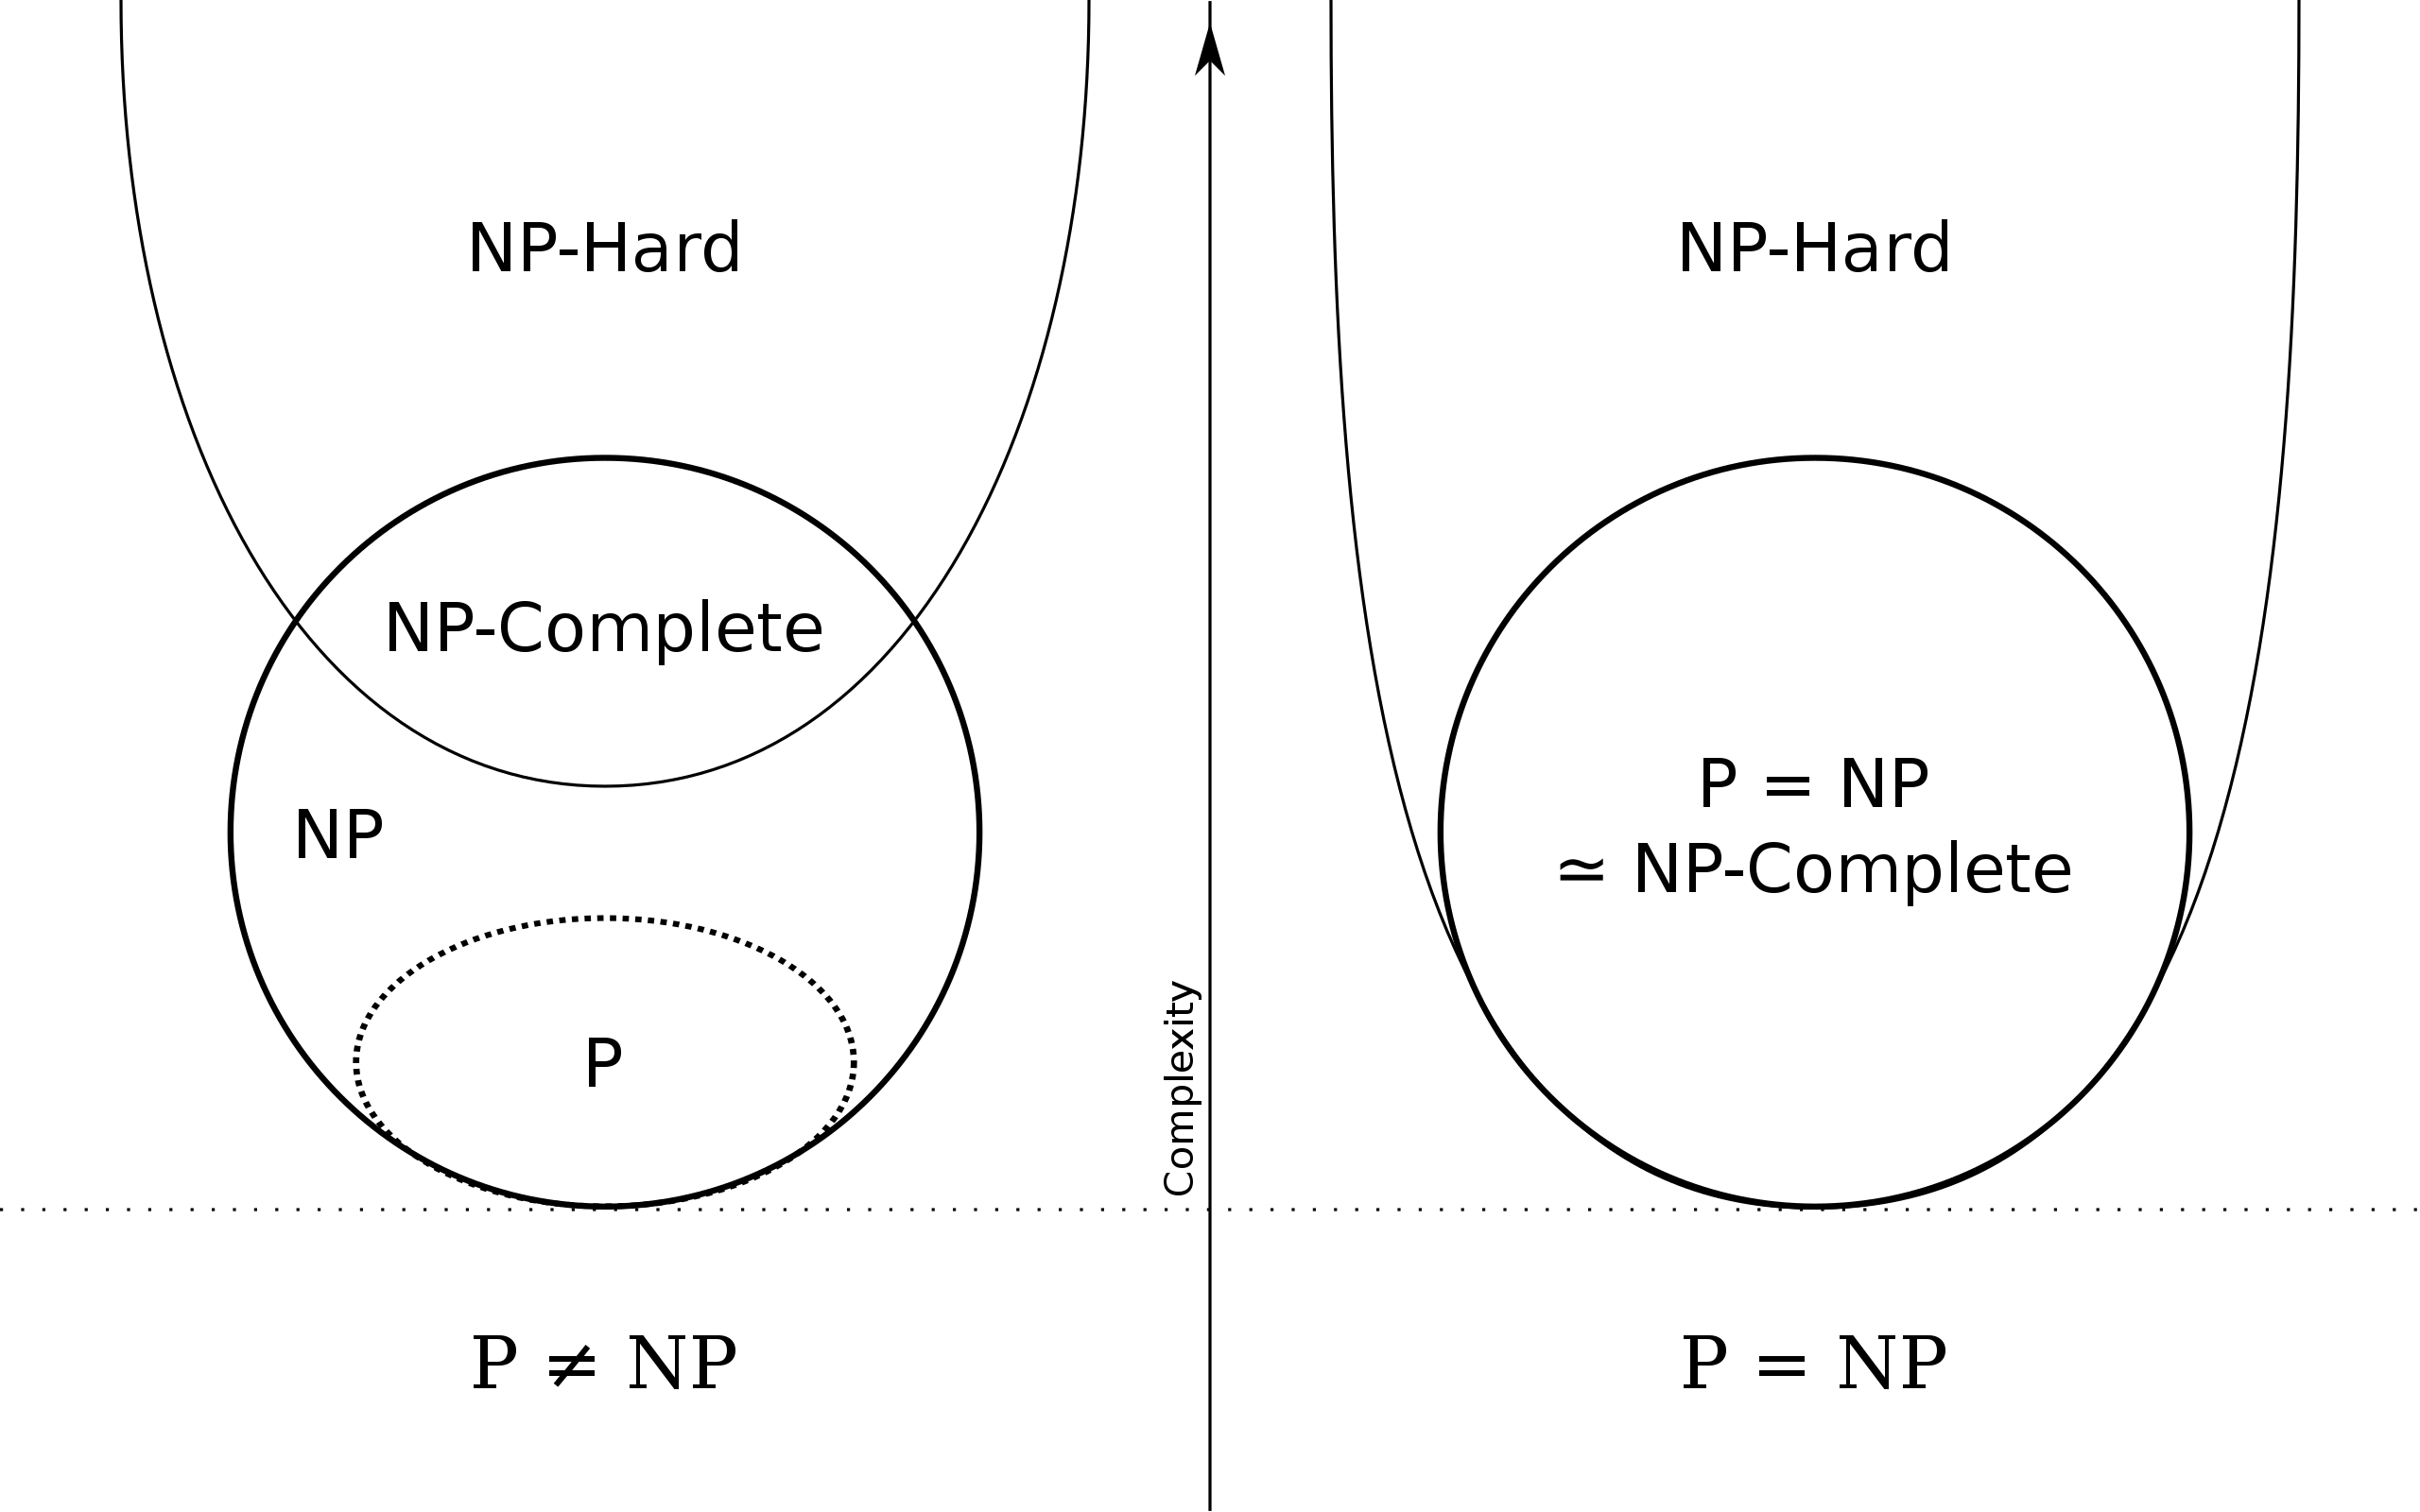
\includegraphics[width=0.9\textwidth]{p2.png}
    \end{center} 
    
    
    \item \ [8 pts] Set up a table to compute the length of the Longest Common Subsequence for the following two strings:
    \begin{align*}
        A \ C \ T \ T \ C \ G \ C \ C \ and \ C \ T \ A \ C \ G \ A \ C
    \end{align*}
    \begin{sol}
    5
    \end{sol}

    \item \ [6 pts] Two people need to establish a secret key for encrypting communications. They agree to use a Diffie-Hellman key exchange with a modulus of 11 and decide on 2 as the base. Person A chooses a random value of 9 and performs the appropriate computations. Person B chooses a random value of 3 and performs the appropriate computations:
    \begin{enumerate}
        \item What is the value Person A sends to Person B
        \begin{sol}
            6
        \end{sol}
        \item What is the value Person B sends to Person A
        \begin{sol}
            8
        \end{sol}
        \item What is the shared secret key between Person A and Person B
        \begin{sol}
            7
        \end{sol}
    \end{enumerate}
    \item \ \textcolor{red}{[8 pts] You have 5 different dice. The table for the summation of the dice is listed below for die 1,2 and 3. Die \#4 has 4 sides of values \{1, 2, 3, 4\} and Die \#5 has 4 sides of values \{-1, -1, 0, 0\}.}
    \begin{enumerate}
        \item Fill in the table for Die 4 and Die 5.
                \begin{center}
    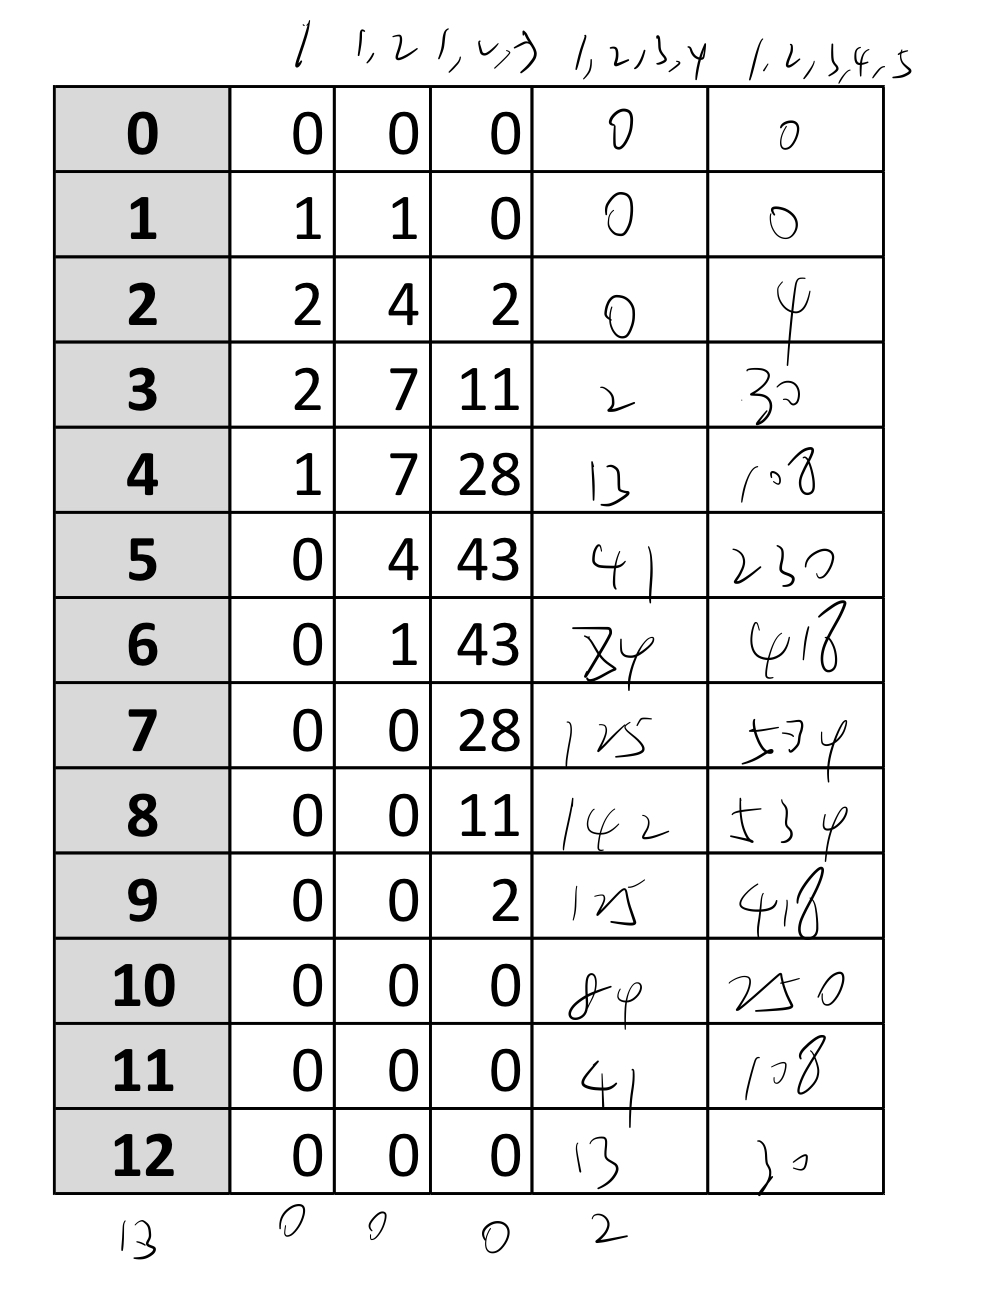
\includegraphics[width=0.4\textwidth]{p5.jpeg}
    \end{center} 
        \item How many sides and of what values is Die \#1?
        6 sides, value is 1, 2, 2, 3, 3, 4
        \item What is the probability of rolling a 6 with these dice?
        \begin{sol}
            \begin{align*}
                \frac{418}{(2+11+28+43+43+28+11+2) \times 4\times4}=\frac{418}{168 \times 16} = \frac{418}{2688}\approx0.156
            \end{align*}
        \end{sol}
        
    \end{enumerate}

    \item \ [10 pts] Determine a Huffman encoding for each symbol in a message that contains:
        \begin{center}
    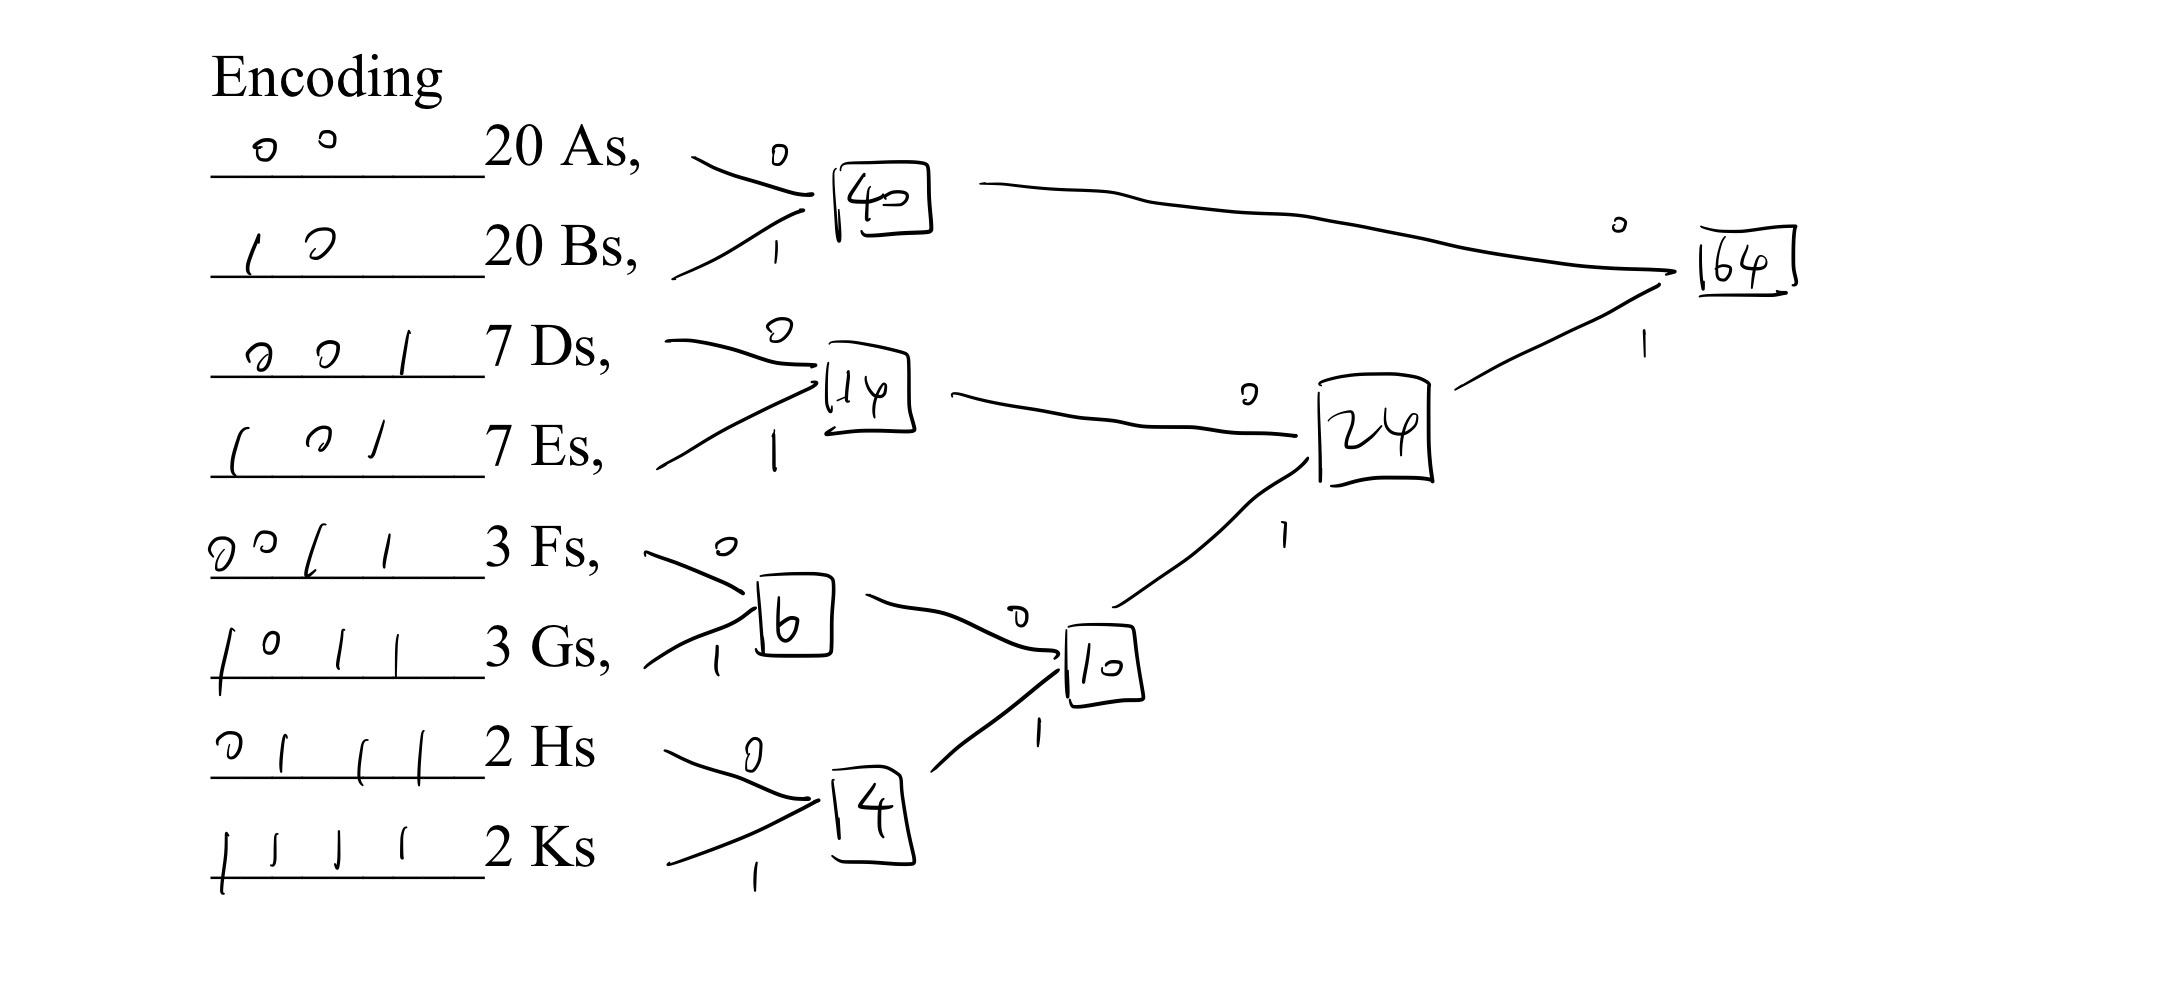
\includegraphics[width=0.9\textwidth]{p3.jpeg}
    \end{center} 
    \begin{enumerate}
        \item How many bits are in the entire message if each symbol is encoded with 3 bits?
        \begin{sol}
            192 bits
        \end{sol}
        \item How many bits are in the entire Huffman coded message?
        \begin{sol}
            162 bits
        \end{sol}
        \item How much entropy is in the entire message (Give a number)?
        \begin{sol}
            158.35 bits
        \end{sol}
    \end{enumerate}


    \item \ [6 pts] Argue that the problem of sorting an array of numbers is just as hard or possibly harder (within $\Theta(1)$ ) than the problem of finding a median of an array of numbers.
    \begin{sol}
        Since we can use a solver for problem of finding a median of array of numbers by sorting an array of numbers, Problem of sorting an array of numbers is just as hard or possibly harder (within $\Theta(1)$) than the problem of finding a median of an array of numbers: sorting array + pick the median($\Theta(1)$)
    \end{sol}

    \item \ [5 pts] A rooted tree has an
    \begin{enumerate}
        \item In-order Traversal of X Q K H N F M W B Y G P D S Z
        \item Pre-Order Traversal of G M H Q X K N F Y M B P D Z S
    \end{enumerate}
Draw the Tree
        \begin{center}
    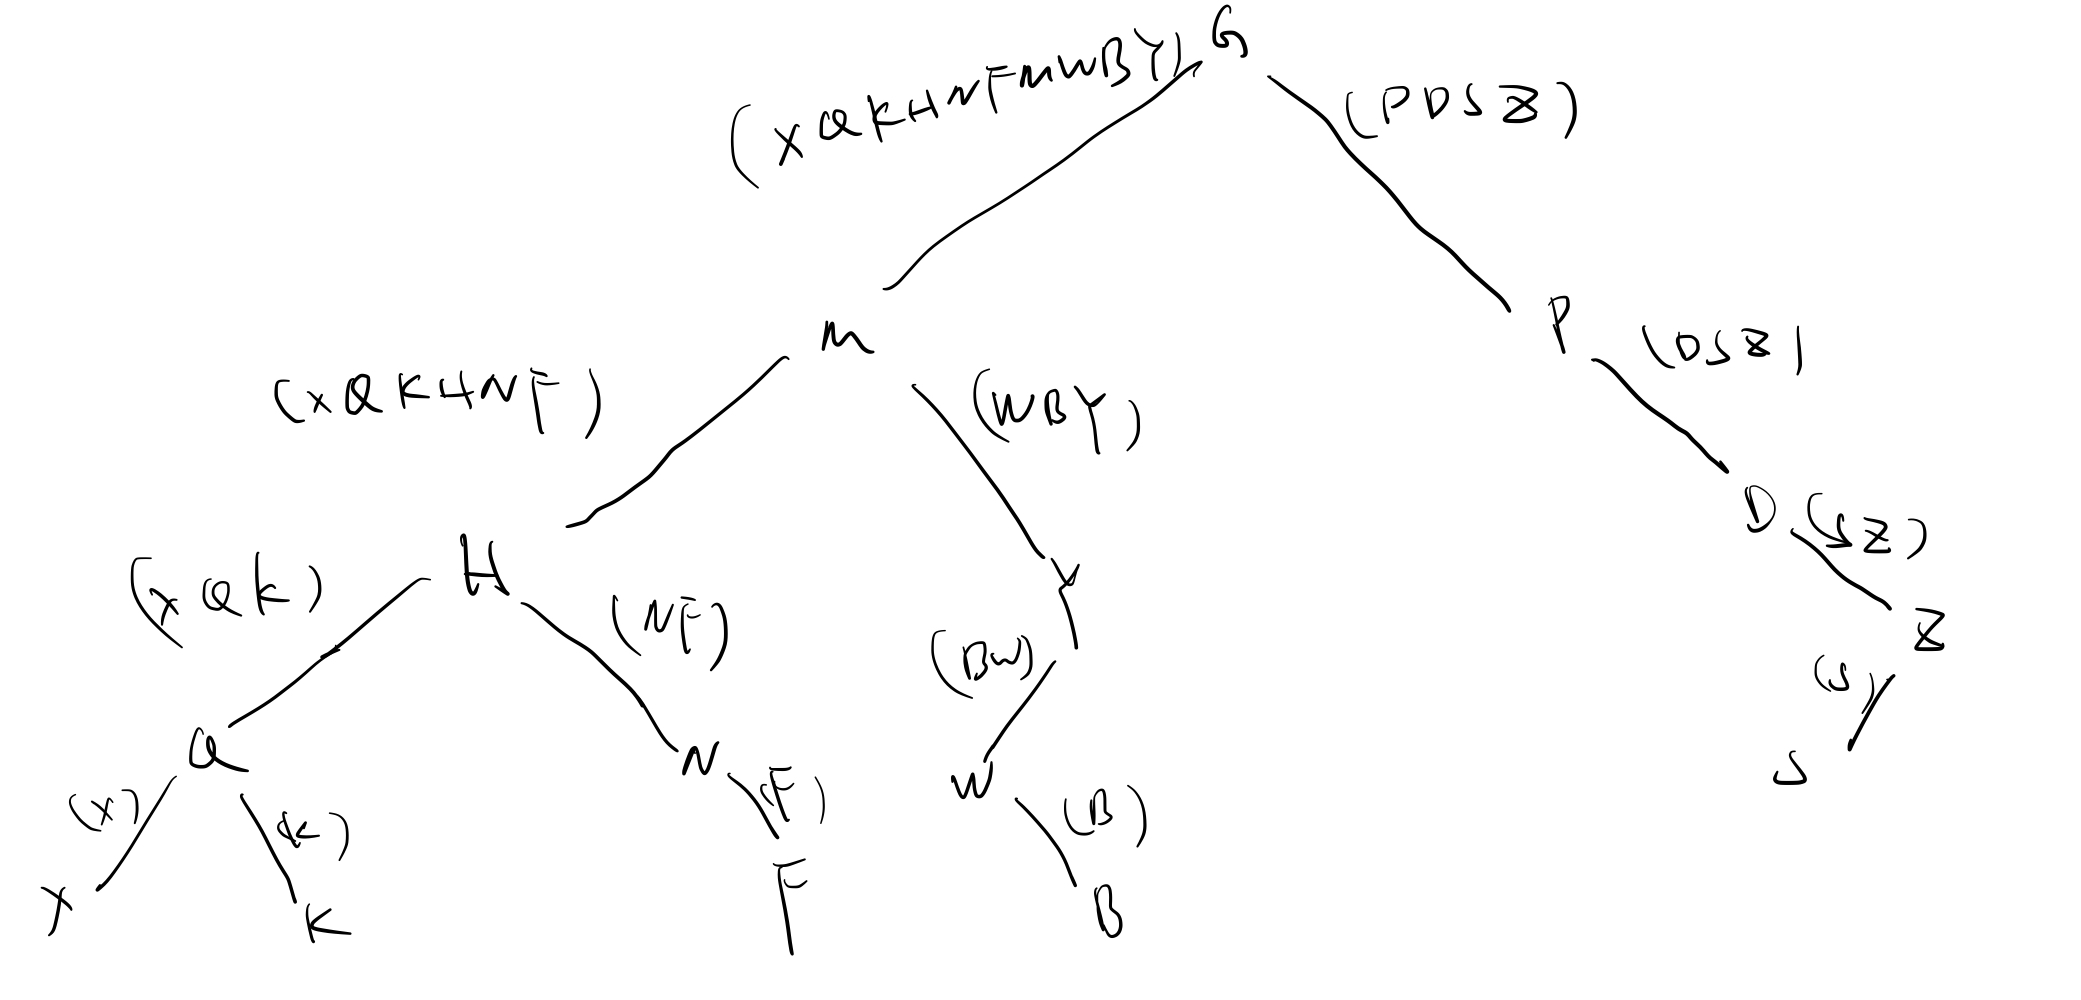
\includegraphics[width=0.9\textwidth]{p4.jpeg}
    \end{center} 

\item \ [9 pts] A complete bi-partite graph $B_{j,k}$ is a graph which has j vertices in one partition and k vertices in another partition and all possible edges are present. Answer the following questions:
\begin{enumerate}
    \item \textcolor{red}{For which values of j and k does $B_{j,k}$ have an Euler Tour?}
    \begin{sol}
        even $j$ and even $k$.
    \end{sol}
    \item For which values of j and k is $B_{j,k}$ two-colorable?
    \begin{sol}
        all
    \end{sol}
    \item \textcolor{red}{For which values of j and k is $B_{j,k}$ a tree?}
    \begin{sol}
        j or k = 1
    \end{sol}
    \item If every edge of tree of $B_{j,k}$ has a weight of w, what is the weight of the minimum spanning tree of $B_{j,k}$
    \begin{sol}
        (j + k - 1) w
    \end{sol}
    \item If every edge of tree of $B_{j,k}$ has a weight of w, what is the maximum flow between the two partitions of $B_{j,k}$
    \begin{sol}
        jkw
    \end{sol}
    \item \textcolor{red}{For which values of j and k does $B_{j,k}$ have a Hamiltonian Cycle?}
    \begin{sol}
        j = k
    \end{sol}
    
\end{enumerate}

\item \ [10 pts] Consider an RSA encryption system that has a public key of 1109 for the value of e and 2881 for the value of the modulus n. A message was encrypted with this key and this encrypted message has the value 2.
\begin{enumerate}
    \item \ [6 pts] With a quantum computer, you were able to factor the modulus 2881 into the product of two primes: 43*67. Using this information, determine the private key. Be sure to show your table for the Extended Euclidian Algorithm
    \begin{sol}
        d = 5; private = (5, 2881)
    \end{sol}
    \item \ [2 pts] What is the unencrypted message?
    \begin{sol}
        32
    \end{sol}
\end{enumerate}

\item \ \textcolor{red}{ [6 pts] Answer the Following:}
\begin{enumerate}
    \item -3 mod 7 = 
    \begin{sol}
        4
    \end{sol}
    \item 1/3 mod 11 = 
    \begin{sol}
        \begin{align*}
            &(\frac{1}{3} \times 3)  \bmod 11 = 1 \\
            &(4 \times 3) \bmod 11 = 1 \\
            & (\frac{1}{3}) \bmod 11 = 4
        \end{align*}
    \end{sol}
    \item – ( 1/3 ) mod 13 =
    \begin{sol}
        \begin{align*}
            &(-\frac{1}{3} \times 3) \bmod 13 = -1 \bmod 13 = 12\\
            &(4\times 3) \bmod 13 = 12 \\
            &-\frac{1}{3} \bmod 13 = 4 \\
        \end{align*}
    \end{sol}
    \item $2^{122} \bmod 11 =$
    \begin{sol}
        \begin{align*}
            & 2^{122} \bmod 11 = 2\times2^{121} \bmod 11\\
            & = 2 \times (2^{11})^{11} \bmod 11 \\
            & = 2 \times (2^{11} \bmod 11) ^{11} \bmod 11\\
            & = 2 \times 2^{11} \bmod 11\\
            & = 2 \times 2 \\
            & = 4 \\
        \end{align*}
    \end{sol}
    \item $1 \bar{4} $ base $8 = $ \underline{ \ \ \ \ \ \ \ \ } base $10$. 
    \begin{sol}
    \begin{align*}
        1 \times 8 ^ 1 + (-4) \times 8^0 = 8 -4 = 4
    \end{align*}
    \end{sol}
    \item A message has 160 symbols in it. The symbol Z occurs 10 times. How much entropy does each ‘Z’ contain in the message?
    \begin{sol}
        \begin{align*}
            \log_{2}\frac{1}{\frac{10}{160}} = \log_2 (16) = \log_2(2^4) = 4
        \end{align*}
    \end{sol}
    \item  What is the length of the longest common subsequence of the two strings: AABBBBCC and ZZBBBBYY
    \begin{sol}
        4
    \end{sol}
    \item What are the maximum number of swaps might be necessary to insert an element into a heap that has 16 elements in it already?
    \begin{sol}
        \begin{align*}
            log_2(16) = 4
        \end{align*}
    \end{sol}
    \item What is $2 + 2$?
    \begin{sol}
        4
    \end{sol}
\end{enumerate}
\end{enumerate}
\end{document}
